%----------
%	CONFIGURACIÓN DEL DOCUMENTO
%----------

% Definimos las características del documento y añadimos una serie de paquetes (\usepackage{package}) que agregan funcionalidades a LaTeX.

\documentclass[12pt]{report} %fuente a 12pt

% MÁRGENES: 2,5 cm sup. e inf.; 3 cm izdo. y dcho.
\usepackage[
a4paper,
vmargin=2.5cm,
hmargin=3cm
]{geometry}

% INTERLINEADO: Estrecho (6 ptos./interlineado 1,15) o Moderado (6 ptos./interlineado 1,5)
\renewcommand{\baselinestretch}{1.15}
\parskip=6pt

% DEFINICIÓN DE COLORES para portada y listados de código
\usepackage[table]{xcolor}
\definecolor{azulUC3M}{RGB}{0,0,102}
\definecolor{gray97}{gray}{.97}
\definecolor{gray75}{gray}{.75}
\definecolor{gray45}{gray}{.45}

% Soporte para GENERAR PDF/A --es importante de cara a su inclusión en e-Archivo porque es el formato óptimo de preservación y a la generación de metadatos, tal y como se describe en http://uc3m.libguides.com/ld.php?content_id=31389625. En la carpeta incluímos el archivo plantilla_tfg_2017.xmpdata en el que puedes incluir los metadatos que se incorporarán al archivo PDF cuando lo compiles. Ese archivo debe llamarse igual que tu archivo .tex. Puedes ver un ejemplo en esta misma carpeta.
\usepackage[a-1b]{pdfx}

% ENLACES
\usepackage{hyperref}
\hypersetup{colorlinks=true,
	linkcolor=black, % enlaces a partes del documento (p.e. índice) en color negro
	urlcolor=blue} % enlaces a recursos fuera del documento en azul

% EXPRESIONES MATEMATICAS
\usepackage{amsmath,amssymb,amsfonts,amsthm}

\usepackage{txfonts} 
\usepackage[T1]{fontenc}
\usepackage[utf8]{inputenc}

\usepackage[spanish, es-tabla]{babel} 
\usepackage[babel, spanish=spanish]{csquotes}
\usepackage{etoolbox}
\AtBeginEnvironment{quote}{\small}

% diseño de PIE DE PÁGINA
\usepackage{fancyhdr}
\pagestyle{fancy}
\fancyhf{}
\renewcommand{\headrulewidth}{0pt}
\rfoot{\thepage}
\fancypagestyle{plain}{\pagestyle{fancy}}

% DISEÑO DE LOS TÍTULOS de las partes del trabajo (capítulos y epígrafes o subcapítulos)
\usepackage{titlesec}
\usepackage{titletoc}
\titleformat{\chapter}[block]
{\large\bfseries\filcenter}
{\thechapter.}
{5pt}
{\MakeUppercase}
{}
\titlespacing{\chapter}{0pt}{0pt}{*3}
\titlecontents{chapter}
[0pt]                                               
{}
{\contentsmargin{0pt}\thecontentslabel.\enspace\uppercase}
{\contentsmargin{0pt}\uppercase}                        
{\titlerule*[.7pc]{.}\contentspage}                 

\titleformat{\section}
{\bfseries}
{\thesection.}
{5pt}
{}
\titlecontents{section}
[5pt]                                               
{}
{\contentsmargin{0pt}\thecontentslabel.\enspace}
{\contentsmargin{0pt}}
{\titlerule*[.7pc]{.}\contentspage}

\titleformat{\subsection}
{\normalsize\bfseries}
{\thesubsection.}
{5pt}
{}
\titlecontents{subsection}
[10pt]                                               
{}
{\contentsmargin{0pt}                          
	\thecontentslabel.\enspace}
{\contentsmargin{0pt}}                        
{\titlerule*[.7pc]{.}\contentspage}  


% DISEÑO DE TABLAS. Puedes elegir entre el estilo para ingeniería o para ciencias sociales y humanidades. Por defecto, está activado el estilo de ingeniería. Si deseas utilizar el otro, comenta las líneas del diseño de ingeniería y descomenta las del diseño de ciencias sociales y humanidades
\usepackage{multirow} % permite combinar celdas 
\usepackage{caption} % para personalizar el título de tablas y figuras
\usepackage{floatrow} % utilizamos este paquete y sus macros \ttabbox y \ffigbox para alinear los nombres de tablas y figuras de acuerdo con el estilo definido. Para su uso ver archivo de ejemplo 
\usepackage{array} % con este paquete podemos definir en la siguiente línea un nuevo tipo de columna para tablas: ancho personalizado y contenido centrado
\newcolumntype{P}[1]{>{\centering\arraybackslash}p{#1}}
\DeclareCaptionFormat{upper}{#1#2\uppercase{#3}\par}

% Diseño de tabla para ingeniería
\captionsetup[table]{
	format=upper,
	name=TABLA,
	justification=centering,
	labelsep=period,
	width=.75\linewidth,
	labelfont=small,
	font=small,
}

%Diseño de tabla para ciencias sociales y humanidades
%\captionsetup[table]{
%	justification=raggedright,
%	labelsep=period,
%	labelfont=small,
%	singlelinecheck=false,
%	font={small,bf}
%}


% DISEÑO DE FIGURAS. Puedes elegir entre el estilo para ingeniería o para ciencias sociales y humanidades. Por defecto, está activado el estilo de ingeniería. Si deseas utilizar el otro, comenta las líneas del diseño de ingeniería y descomenta las del diseño de ciencias sociales y humanidades
\usepackage{graphicx}
\graphicspath{{res/}} %ruta a la carpeta de imágenes

\usepackage{afterpage}
% Diseño de figuras para ingeniería
\captionsetup[figure]{
	format=hang,
	name=Fig.,
	singlelinecheck=off,
	labelsep=period,
	labelfont=small,
	font=small		
}


% NOTAS A PIE DE PÁGINA
\usepackage{chngcntr} %para numeración contínua de las notas al pie
\counterwithout{footnote}{chapter}

% LISTADOS DE CÓDIGO
% soporte y estilo para listados de código. Más información en https://es.wikibooks.org/wiki/Manual_de_LaTeX/Listados_de_código/Listados_con_listings
\usepackage{listings}

% definimos un estilo de listings
\lstdefinestyle{estilo}{ frame=Ltb,
	framerule=0pt,
	aboveskip=0.5cm,
	framextopmargin=3pt,
	framexbottommargin=3pt,
	framexleftmargin=0.4cm,
	framesep=0pt,
	rulesep=.4pt,
	backgroundcolor=\color{gray97},
	rulesepcolor=\color{black},
	%
	basicstyle=\ttfamily\footnotesize,
	keywordstyle=\bfseries,
	stringstyle=\ttfamily,
	showstringspaces = false,
	commentstyle=\color{gray45},     
	%
	numbers=left,
	numbersep=15pt,
	numberstyle=\tiny,
	numberfirstline = false,
	breaklines=true,
	xleftmargin=\parindent
}

\captionsetup[lstlisting]{font=small, labelsep=period}
% fijamos el estilo a utilizar 
\lstset{style=estilo}
\renewcommand{\lstlistingname}{\uppercase{Código}}


%BIBLIOGRAFÍA - PUEDES ELEGIR ENTRE ESTILO IEEE O APA. POR DEFECTO ESTÁ CONFIGURADO IEEE. SI DESEAS USAR APA, COMENTA LAS LÍNEA DE IEEE Y DESCOMENTA LAS DE APA. Si haces cambios en la configuración de la bibliografía y no obtienes los resultados esperados, es recomendable limpiar los archivos auxiliares y volver a compilar en este orden: COMPILAR-BIBLIOGRAFIA-COMPILAR

% Tienes más información sobre cómo generar bibliografía y CONFIGURAR TU EDITOR DE TEXTO para compilar con biber en http://tex.stackexchange.com/questions/154751/xx-with-biber-configuring-my-editor-to-avoid-undefined-citations , https://www.overleaf.com/learn/latex/Bibliography_management_in_LaTeX y en http://www.ctan.org/tex-archive/macros/latex/exptl/biblatex-contrib
% También te recomendamos consultar la guía temática de la Biblioteca sobre citas bibliográficas: http://uc3m.libguides.com/guias_tematicas/citas_bibliograficas/inicio

% CONFIGURACIÓN PARA LA BIBLIOGRAFÍA IEEE
\usepackage[backend=biber, style=ieee, isbn=false,sortcites, maxbibnames=5, minbibnames=1]{biblatex} % Configuración para el estilo de citas de IEEE, recomendado para el área de ingeniería. "maxbibnames" indica que a partir de 5 autores trunque la lista en el primero (minbibnames) y añada "et al." tal y como se utiliza en el estilo IEEE.

% Añadimos las siguientes indicaciones para mejorar la adaptación de los estilos en español
\DefineBibliographyStrings{spanish}{%
	andothers = {et\addabbrvspace al\adddotspace}
}
\DefineBibliographyStrings{spanish}{
	url = {\adddotspace[En línea]\adddotspace Disponible en:}
}
\DefineBibliographyStrings{spanish}{
	urlseen = {Acceso:}
}
\DefineBibliographyStrings{spanish}{
	pages = {pp\adddotspace},
	page = {p.\adddotspace}
}


\addbibresource{bib/bibliography.bib} % llama al archivo bibliografia.bib en el que debería estar la bibliografía utilizada

% my settings
\linespread{1.5}
\usepackage{float}
\usepackage[bottom]{footmisc}
\usepackage{enumitem}
\newcommand{\sigmadelta}{$\Sigma\Delta\; $}
\usepackage{microtype}

%-------------
%	DOCUMENTO
%-------------

\begin{document}
\pagenumbering{roman} % Se utilizan cifras romanas en la numeración de las páginas previas al cuerpo del trabajo

%----------
%	PORTADA
%----------	
\begin{titlepage}

	\begin{sffamily}
	\color{azulUC3M}
	\begin{center}
		\begin{figure}[H] %incluimos el logotipo de la Universidad
			\makebox[\textwidth][c]{
\includegraphics[width=16cm]{res/Portada_Logo.png}}
		\end{figure}
		\vspace{2.5cm}
		\begin{Large}
			Grado en Ingeniería en Tecnologías Industriales		
			2019-2020
			\vspace{2cm}		
			\textsl{Trabajo de Fin de Grado}
			\bigskip
			
		\end{Large}
		 	{\Huge LINEALIZACIÓN DE OSCILADOR EN ANILLO CONTROLADO POR TENSIÓN MEDIANTE CAPACIDADES CONMUTADAS}\\
		 	\vspace*{0.5cm}
	 		\rule{10.5cm}{0.1mm}\\
			\vspace*{0.9cm}
			{\LARGE Roberto Uceda Gómez}\\ 
			\vspace*{1cm}
		\begin{Large}
			Tutor:
			Eric Gutiérrez Fernández
			Leganés, {fecha}
		\end{Large}
	\end{center}
	\vfill
	\color{black}
	% si nuestro trabajo se va a publicar con una licencia Creative Commons, incluir estas líneas. Es la opción recomendada.
	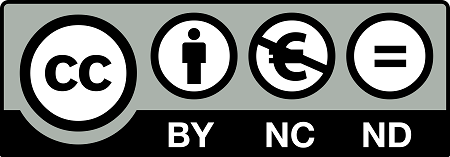
\includegraphics[width=4.2cm]{res/creativecommons.png}\\ %incluimos el logotipo de creativecommons
	Esta obra se encuentra sujeta a la licencia Creative Commons\\ \textbf{Reconocimiento - No Comercial - Sin Obra Derivada}
	\end{sffamily}
\end{titlepage}

\newpage %página en blanco o de cortesía
\thispagestyle{empty}
\mbox{}

%----------
%	RESUMEN Y PALABRAS CLAVE
%----------	
\renewcommand\abstractname{\large\bfseries\filcenter\uppercase{Resumen}}
\begin{abstract}
\thispagestyle{plain}
\setcounter{page}{3}
	
	% ESCRIBIR EL RESUMEN AQUÍ
	En este trabajo se desarrolla un estudio cuyo objetivo es el diseño de una nueva arquitectura de convertidor analógico digital por oscilador controlado por tensión que reduzca el ruido y el consumo en comparación con las arquitecturas habituales.
	
	\textbf{Palabras clave: ADC-VCO, Oscilador en anillo, Conversión Analógico-Digital, CMOS}
	% Escribir las palabras clave aquí
	
	TODO
	\vfill
\end{abstract}
	\newpage % página en blanco o de cortesía
	\thispagestyle{empty}
	\mbox{}


%----------
%	DEDICATORIA
%----------	
\chapter*{Dedicatoria}

\setcounter{page}{5}
	
	TODO
		
	\vfill
	
	\newpage % página en blanco o de cortesía
	\thispagestyle{empty}
	\mbox{}
	

%----------
%	ÍNDICES
%----------	

%--
% Índice general
%-
\tableofcontents
\thispagestyle{fancy}


%--
% Índice de figuras. Si no se incluyen, comenta las líneas siguientes
%-
\listoffigures
\thispagestyle{fancy}


%--
% Índice de tablas. Si no se incluyen, comenta las líneas siguientes
%-
\listoftables
\thispagestyle{fancy}


%--
% Lista de abreviaturas. Si no se incluyen, comenta las líneas siguientes
%-
\newpage
\begin{table}[h!]
	\setlength{\arrayrulewidth}{0mm}
	\begin{center}
		\caption{Lista de abreviaturas}
		\label{tab:table1}
		\begin{tabular}{>{\bf}p{4cm}|p{10cm}}
			ADC & Analog to Digital Converter, Convertidor Analógico-Digital \\
			CMOS & Complimentary Metal-Oxide Semiconductor \\
			MOSFET & Metal Oxide Semiconductor Field Effect Transistor, también llamados transistores MOS \\
		\end{tabular}
	\end{center}
\end{table}

\newpage % página en blanco o de cortesía
\thispagestyle{empty}
\mbox{}

%----------
%	TRABAJO
%----------	
\clearpage
\pagenumbering{arabic} % numeración con múmeros arábigos para el resto de la publicación	

\chapter{Introducción}

	Los convertidores ADC\footnote{Analog to Digital Converter. En español, Convertidor Analógico a Digital} son onmipresentes en nuestro día a día. Sin ellos, no sería posible realizar una llamada con un teléfono móvil, o disfrutar de un sistema de climatización en nuestro hogar, o utilizar el control de crucero en nuestro coche. El objetivo de estos importantes bloques de la electrónica es convertir señales físicas, como ondas electromagnéticas, temperatura ambiente, o la posición de un eje, en señales digitales interpretables por un sistema basado en la electrónica digital. Una vez tenemos estas señales, normalmente compuestas por un flujo de bits, pueden ser procesadas por un microcontrolador para después tomar las decisiones necesarias para conseguir el objetivo deseado, como activar el compresor del aire acondicionado si la temperatura sube de cierto límite preestablecido.
	
	Cada día que pasa aumenta la demanda de aparatos más rápidos, compactos, y eficientes. Por regla general, la miniaturización de la electrónica tiene un impacto positivo en estos criterios. Los transistores son los componentes fundamentales de los circuitos integrados, donde recae el grueso de consumo y tamaño en un sistema electrónico. Estos transistores aumentan su eficiencia energética según disminuye su tamaño, además de permitir mayores frecuencias de operación. Por esto, existe un gran incentivo en la búsqueda de arquitecturas y técnicas de fabricación que permitan transistores más pequeños.
	
	La ley de Moore ayuda a poner un poco de contexto histórico a esta carrera por la disminución de los transistores. Gordon Moore anunció en 1965 una tendencia en la, por aquel entonces emergente, industria de la electrónica: cada dos años se duplicaba la cantidad de componentes presente en un circuito integrado en la misma superficie \cite{moorelaw}. A más componentes, mayor poder de procesamiento, pero también mayor coste de fabricación por la complejidad y delicadeza requerida en los procesos.
	
	\section{Motivación del trabajo}
	
	Debido a las altas velocidades de reloj y los requisitos de consumo y fabricación (espacio ocupado, número de componentes), los ADC usados actualmente presentan problemas. Los ADC basados en la arquitectura sigma delta necesitan un amplificador operacional a modo de integrador. Los ADC basados en VCO actuales, o bien necesitan un integrador de manera similar a los sigma-delta, o bien necesitan una compensación de linearidad mediante circuitería digital. Los amplificadores operacionales y los circuitos de compensación requieren de mucho espacio y gran número de componentes, además de consumir más de lo deseable. Este trabajo se centra en la búsqueda de una nueva arquitectura usando un VCO tanto como integrador como cuantificador, que permita ahorrar la necesidad de circuitos de compensación o amplificadores operacionales, manteniendo o mejorando el comportamiento lineal, la resolución, y el ancho de banda de las arquitecturas ya existentes.
	
	\section{Objetivos}
	
	El grueso de este trabajo se encuentra en el plano teórico. El primer paso es realizar un estudio de las arquitecturas de ADC ya existentes, centrándose en aquellas que emplean VCOs. A partir de este estudio, se estudiará la viabilidad de varias ideas de diferentes publicaciones que aún no han sido implementadas. Para esto, se utilizarán herramientas de simulación basadas en SPICE. Una vez probada la efectividad de la arquitectura, la siguiente tarea será montar un circuito con componentes discretos sobre protoboard, medir los parámetros de funcionamiento, y así dejar demostrada la factibilidad de la arquitectura.
	TODO: consultar Eric

	\section{Marco regulador}
	TODO	
	preguntar a Eric
	
	
	\section{Esquema de este documento}
	TODO
	por decidir
	

	
	

\chapter{Estado del arte}

	Para entender las arquitecturas de ADC modernas es imprescindible conocer primero los bloques fundamentales sobre los que se asienta la microelectrónica actualmente: los transistores MOSFET\footnote{Metal Oxide Semiconductor Field Effect Transistor}.
	
	\section{Transistores MOS}
	
	\begin{figure}[H]
		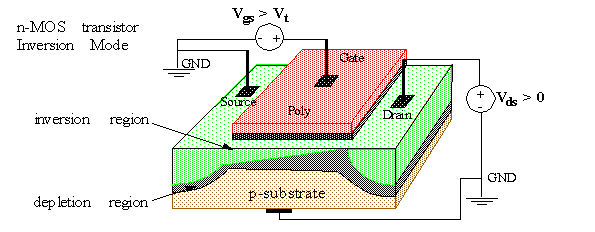
\includegraphics[width=\textwidth]{mos_transistor.png}
		\caption[Corte de transistor MOSFET]{Corte de transistor MOSFET\protect\footnotemark}
		\label{fig:mos_transistor.png}
	\end{figure}

	\footnotetext{Fuente: \url{http://ece-research.unm.edu/jimp/vlsi/slides/chap2_1.html} }
	
	Un transistor MOSFET es un tipo de transistor bipolar que se usa para amplificar y conmutar señales eléctricas dentro de un circuito. Se compone de cuatro entradas: fuente, puerta, drenador, y sustrato, que normalmente está conectado a la fuente. Cuando se aplica un voltaje en la puerta, se crea un canal en el medio semiconductor que permite el paso de corriente entre la fuente y el drenador. Podemos distinguir dos tipos de transistores MOS: los canal-n y los canal-p, dependiendo del dopaje del silicio usado en su fabricación. Los canal-n tienen un dopaje negativo en el silicio de la fuente y el drenador, que se consigue añadiendo impurezas de un elemento como fósforo, dejando electrones libres que actúan como portadores de carga. En el caso de los canal-p, se dopan con elementos como boro, que dejan huecos (ausencia de electrones en capas de valencia), y estos actúan como portadores de carga.
	
	Estos son los símbolos más usados para representar transistores MOS:
	
	\begin{figure}[H]
		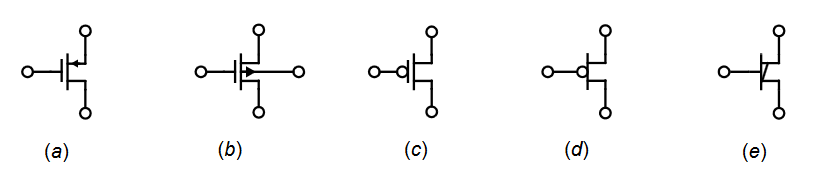
\includegraphics[width=0.8\textwidth]{p-mos-symbol.png}
		\caption[Transistor MOS, canal-p]{Transistor MOS, canal-p\protect\footnotemark}
		\label{fig:p-mos-symbol.png}
	\end{figure}

	\footnotetext{Fuente: Analog Integrated Circuit Design\cite{aicd}}
	
	\begin{figure}[H]
		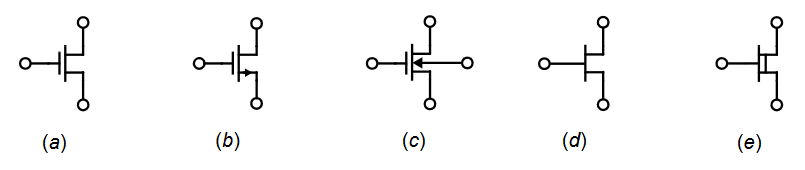
\includegraphics[width=0.8\textwidth]{n-mos-symbol.png}
		\caption[Transistor MOS, canal-n]{Transistor MOS, canal-n\protect\footnotemark}
		\label{fig:n-mos-symbol.png}
	\end{figure}
	
	
	\footnotetext{Fuente: Analog Integrated Circuit Design\cite{aicd}}
	
	\section{Tecnología CMOS}
	
	La tecnología de fabricación CMOS\footnote{Complementary MOS} utiliza una combinación de transistores MOS de canal n y canal p para implementar las funciones de un microprocesador. Por ejemplo, un inversor (puerta lógica NOT) se consigue con la siguiente disposición:
	
	\begin{figure}[H]
		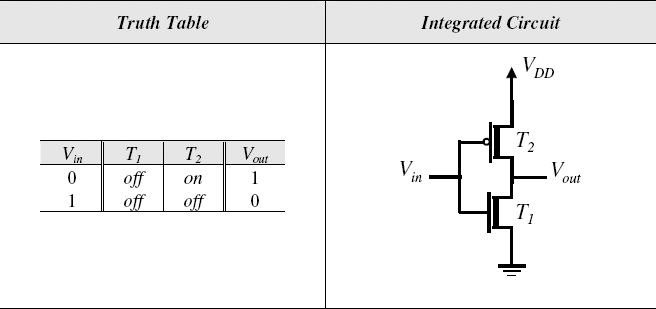
\includegraphics[width=0.75\textwidth]{inverter_mos.jpg}
		\caption[Inversor CMOS]{Inversor CMOS\protect\footnotemark}
		\label{fig:inverter_mos.jpg}
	\end{figure}
	\footnotetext{Fuente: \url{https://www.oreilly.com/library/view/introduction-to-digital/9780470900550/chap5-sec008.html} }
	
	
	Los circuitos CMOS tienen un bajo consumo, tienen una buena resistencia al ruido, y son relativamente fáciles de diseñar. Es por esto que se ha convertido en la tecnología dominante en los microcircuitos.
	
	\section{Conversión analógico-digital}
	
	La tarea de un convertidor analógico-digital, o ADC, es convertir una señal de espectro continuo en el tiempo en una señal de valores discretos cuantizable.
	
	\begin{figure}[H]
		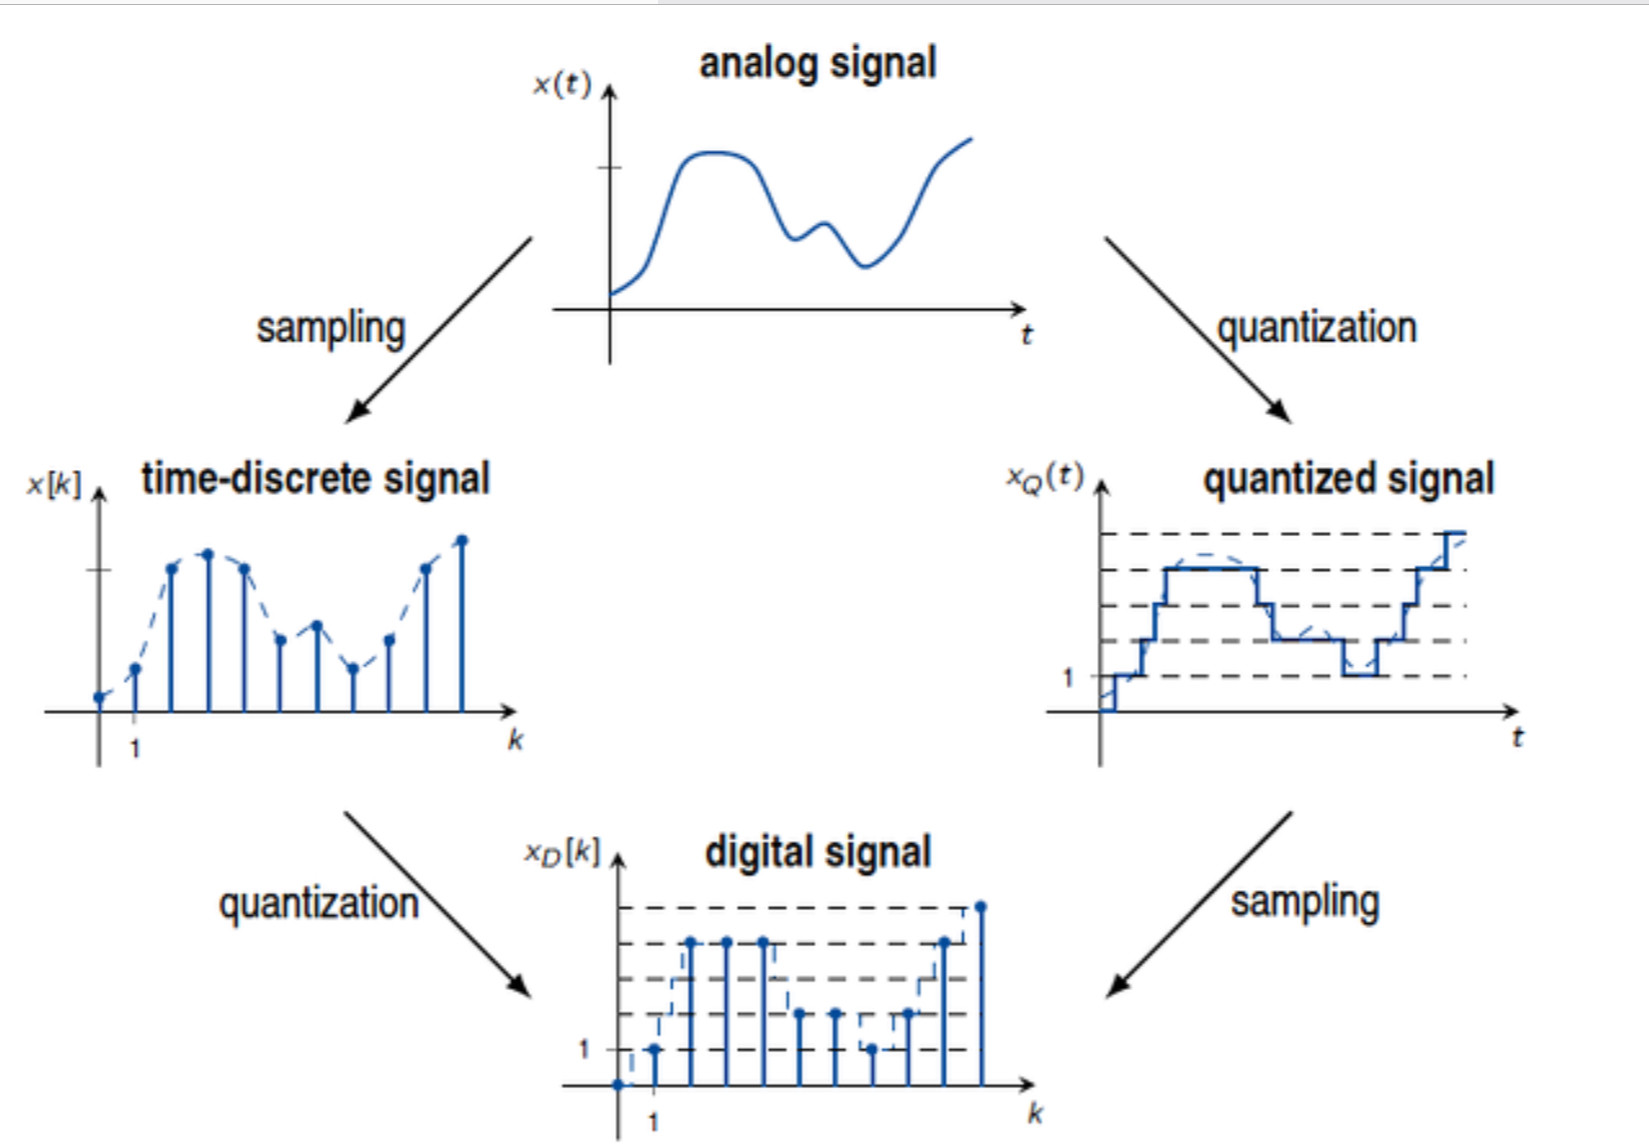
\includegraphics[width=0.75\textwidth]{analog-vs-digital-signal.jpg}
		\caption[Señal analógica a digital]{Señal analógica a digital\protect\footnotemark}
		\label{fig:analog-vs-digital-signal.jpg}
	\end{figure}
	\footnotetext{Fuente: \url{https://electronics.stackexchange.com/questions/352784/in-digital-systems-do-we-discretize-both-time-and-magnitude-or-only-time} }
	
	En un ADC, la señal analógica original sufre dos transformaciones: un muestreo y una cuantificación. El muestro toma valores de la señal a una frecuencia concreta, descartando los intermedios. La cuantificación transforma el espectro continuo de la señal en un conjunto de valores finito. Esto es suficiente para lograr un conjunto de palabras (conjunto de bits de longitud definida) a una frecuencia de trabajo, para ser almacenadas o procesadas por un microcontrolador.
	
	Estos son algunos de los parámetros básicos que describen el comportamiento y prestaciones de un ADC:
	
	\begin{description}[font=\bfseries, style=multiline, align=left, before={\renewcommand\makelabel[1]{\bfseries ##1:}}]
		\item[Frecuencia de muestreo] Frecuencia a la cual se toman medidas de la señal original. Determina el ancho de banda.
		\item[Ancho de banda] Rango de frecuencias de la señal original que puede ser correctamente muestreada, cuantizada, y posteriormente recreada.
		\item[Resolución] Número de pasos máximo entre rango de valores de la señal analógica. Determina el error de cuantificación y el SNR máximo.
		\item[SNR] Signal to Noise Ratio. Relaciona la potencia de la señal de interés y el ruido de fondo existente.
	\end{description}

	En cuanto a errores en la conversión, estas son las principales fuentes:
	
	\begin{description}[font=\bfseries, style=multiline, align=left, before={\renewcommand\makelabel[1]{\bfseries ##1:}}]
		\item[Cuantificación] Para una muestra dada en un momento determinado, diferencia entre el valor de la señal original y valor de la señal cuantificada. Surge porque para cada valor discreto de la señal cuantificada, existe un rango con infinitos valores intermedios en la señal original.
		\item[Linealidad] Falta de correlación lineal entre entrada y salida del ADC. Necesita ser corregida para evitar divergencias entre entrada y salida que distorsionan la lectura.
		\item[Offset] Para valores muy bajos de señal original, la lectura puede ser distorsionada si no se corrige el offset.
		\item[Ganancia] Si no se ajusta correctamente, se puede inducir en un error creciente a medida que se recorre la curva de respuesta.
	\end{description}

	Es importante diferenciar dos tipos de ADC según su frecuencia de muestreo:
	\begin{description}[font=\bfseries, style=multiline, align=left, before={\renewcommand\makelabel[1]{\bfseries ##1:}}]
		\item[A frecuencia de Nyquist] La frecuencia de muestreo es igual a dos veces la frecuencia máxima de la señal a capturar\cite{nyquist}\cite{shannon-nyquist}.
		\item[Sobremuestreados] La frecuencia de muestreo es superior a la frecuencia de Nyquist; habitualmente unas diez veces mayor.
	\end{description}
	
	La mayoría de arquitecturas de ADC actuales trabajan con sobremuestreo, ya que permiten una mejor gestión del ruido.
	
	\section{Arquitecturas de ADC actuales}
	
	Existen multitud de arquitecturas ADC: flash, aproximaciones sucesivas, de integración, de rampa, de seguimiento, tensión-frecuencia, y un largo etcétera.
	
	\begin{figure}[H]
		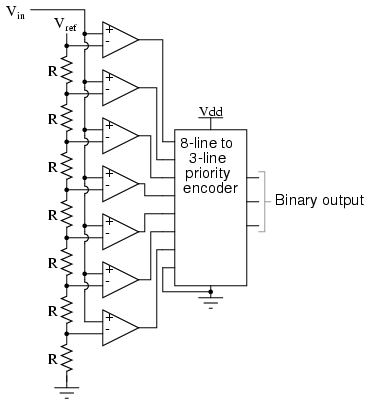
\includegraphics[width=0.5\textwidth]{flash-adc.png}
		\caption[ADC de conversión directa tipo flash]{ADC de conversión directa tipo flash\protect\footnotemark}
		\label{fig:flash-adc.png}
	\end{figure}
	\footnotetext{Fuente: \url{https://www.allaboutcircuits.com/textbook/digital/chpt-13/flash-adc/} }
	\begin{figure}[H]
		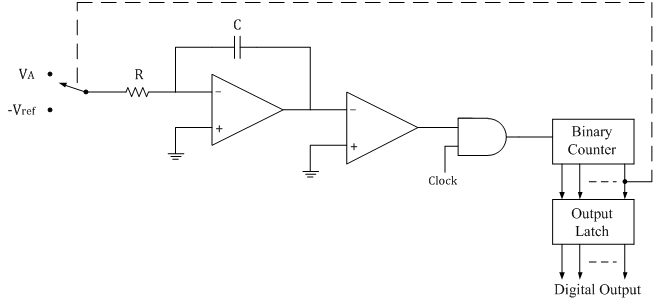
\includegraphics[width=0.6\textwidth]{integrator-adc-double-ramp.png}
		\caption[ADC integrador de doble rampa]{ADC integrador de doble rampa\protect\footnotemark}
		\label{fig:integrator-adc-double-ramp.png}
	\end{figure}
	\footnotetext{Fuente: \url{http://www.electronics-tutorial.net/analog-integrated-circuits/data-converters/dual-slope-type-adc/} }
	
	Los más cercanos a la materia de este estudio son los de integración, en concreto los que utilizan la modulación sigma-delta.
	
	\section{Modulación sigma-delta en ADCs}
	
	Un ADC que utiliza el principio de modulación sigma-delta, también llamado \textit{modulador sigma-delta}, o \textit{modulador \sigmadelta}, tiene como bloques principales un sumador, un integrador, y un cuantificador, además de un bucle de retroalimentación. Este es el esquema de bloques básico de un modulador \sigmadelta:
	
	\begin{figure}[H]
		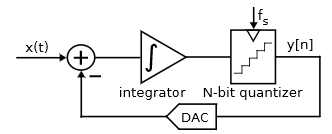
\includegraphics[width=0.6\textwidth]{sigma-delta-blocks.png}
		\caption[Bloques de un modulador \sigmadelta]{Bloques de un modulador \sigmadelta\protect\footnotemark}
		\label{fig:sigma-delta-blocks.png}
	\end{figure}
	\footnotetext{Fuente: Oversampled Analog-To-Digital Converter Architectures Based On Pulse Frequency Modulation\cite{eric-thesis} }
	
	El funcionamiento de este tipo de ADC sigue los pasos siguientes. La señal original \begin{math}( x(t) )\end{math} es sumada a la salida del cuantificador \begin{math}( y(t) )\end{math} en magnitud negativa. La salida \begin{math}( y(t) )\end{math} es un flujo de un bit de profundidad, por lo que debe ser transformada a magnitud real a través de un DAC. El integrador forma un filtro de paso bajo sobre la diferencia entre señal original y cuantificada de tal manera que se consigue una realimentación de baja frecuencia, consiguiendo una reducción del ruido de cuantificación en la banda de respuesta.
	
	Este es un ejemplo gráfico del resultado de la modulación \sigmadelta:
	
	\begin{figure}[H]
		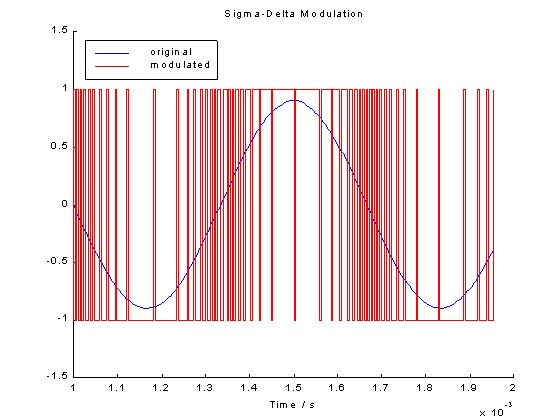
\includegraphics[width=\textwidth]{sd-modulation-example.jpg}
		\caption[Modulación \sigmadelta de una señal de 1.5kHz]{Modulación \sigmadelta de una señal de 1.5kHz\protect\footnotemark}
		\label{fig:sd-modulation-example.jpg}
	\end{figure}

	\footnotetext{Fuente: \url{http://www.cs.tut.fi/sgn/arg/rosti/1-bit/} }
	
	Se puede observar que el promedio de la señal modulada de 1 bit es proporcional a la señal original.
	
	Con respecto a un ADC de aproximaciones sucesivas o de seguimiento, la modulación \sigmadelta una gran linealidad en la curva de respuesta y una disminución del ruido de fondo, ya que el bucle tenderá a hacer que la salida \begin{math} y(t) \end{math} sea cero. El cuantificador suele ser un comparador implementado con un amplificador operacional de alta ganancia, con una referencia ajustada a la aplicación. Además suele existir un circuito sample-and-hold con una frecuencia de reloj que se ajusta a la entrada al circuito que recibirá la señal ya convertida a digital.
	
	Las principales desventajas de la conversión por modulador \sigmadelta son la necesidad de una frecuencia de muestreo muy alta respecto a la original, lo cual es un problema a la hora de convertir señales de muy alta frecuencia;
	TODO: añadir más desventajas
	
	TODO: explicar VCO (o mejor en desarrollo?)

	
\chapter{Análisis}
	
	TODO: nombre para este capítulo
	
	En este capítulo se expone el análisis de una nueva arquitectura de ADC que emplea un VCO como cuantificador e integrador.
	
	\section{Idea inicial}
	
	La idea fundamental de la nueva arquitectura es sustituir el integrador y el cuantificador de un ADC de tipo \sigmadelta por un VCO. Esto eliminaría la necesidad de un amplificador operacional presente en un \sigmadelta, rebajando por tanto el número de componentes necesarios y el consumo total del sistema.
	TODO: preguntar a Eric la fuente original de la idea
	
	El primer paso para desarrollar el estudio es comprender cómo funciona un VCO.
	
	\section{VCO en anillo}
	
	Un VCO, siglas de \textit{Voltage Controlled Oscillator} es un componente electrónico que emite un flujo de pulsos cuya frecuencia es proporcional al voltaje de alimentación.
	
	Un VCO en anillo es un tipo de oscilador controlado por voltaje. En su forma más básica, consiste en un número impar de puertas inversoras colocadas en un bucle. En las entradas de alimentación de las puertas se conecta la señal a modular. La señal ya modulada aparece entre la salida y la entrada de cualquier par de puertas.
	
	Esta es la representación simbólica de una puerta inversora, con sus conexiones nombradas:
	\begin{figure}[H]
		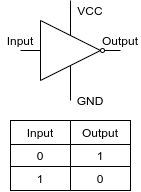
\includegraphics[width=0.3\textwidth]{inverter-symbol.png}
		\caption[Símbolo y tabla de verdad de una puerta inversora]{Símbolo y tabla de verdad de una puerta inversora}
		\label{fig:inverter-symbol.png}
	\end{figure}
	
	Así se consigue un inversor en tecnología CMOS. El transistor superior es de canal-p, y el inferior es de canal-n.
	\begin{figure}[H]
		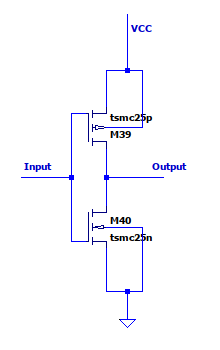
\includegraphics[width=0.4\textwidth]{inverter-sch.png}
		\caption[Esquemático de una puerta inversora con transistores MOS]{Esquemático de una puerta inversora con transistores MOS}
		\label{fig:inverter-sch.png}
	\end{figure}
	
	Cuando la señal de entrada está en cero lógico (0 voltios) el transistor canal-n se encuentra con una diferencia de voltaje baja entre la puerta y la fuente, así que no hay paso de corriente entre la fuente y el drenador. Por su parte, en el transistor canal-p la diferencia de voltaje entre la puerta y la fuente es grande (la fuente está conectada a una fuente de alimentación VCC que proporciona un voltaje llamado bias), así que la corriente entre su fuente y drenador es no nula. Así, en la salida el voltaje es equivalente al voltaje de bias VCC.
	
	Cuando la señal de entrada está en uno lógico (cercano al voltaje de bias), ocurre lo contrario: el transistor n entra en su región activa (permite el paso de corriente) mientras que el p entra en zona de corte (no permite el paso de corriente). Así, la salida estará conectada a tierra, normalmente cero voltios.

	\begin{figure}[H]
		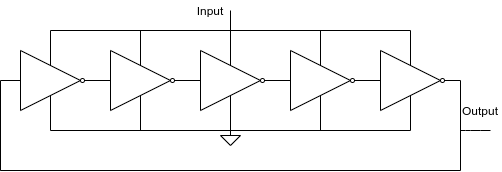
\includegraphics[width=\textwidth]{vco-symbol.png}
		\caption[VCO compuesto por 5 puertas inversoras]{VCO compuesto por 5 puertas inversoras}
		\label{fig:vco-symbol.png}
	\end{figure}

	\begin{figure}[H]
		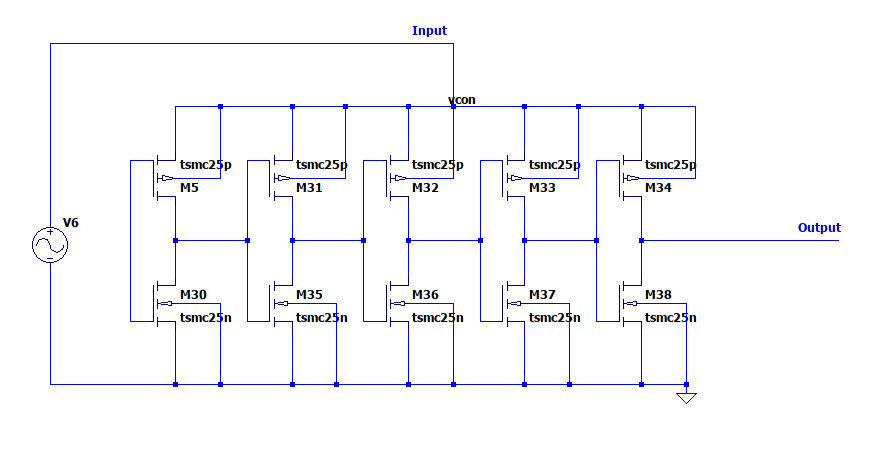
\includegraphics[width=\textwidth]{vco-sch.png}
		\caption[Esquemático de un VCO]{Esquemático de un VCO}
		\label{fig:vco-sch.png}
	\end{figure}

	El número impar de puertas inversoras provoca un estado de inestabilidad en el oscilador. Dado que hay una pequeña demora en la activación de las puertas por (TODO: por qué hay demora en activación?), y por la realimentación positiva en el anillo, se crean señales alternativas entre un 1 lógico y un 0 lógico. La frecuencia a la que estas señales cambian es proporcional al voltaje aplicado en la alimentación de las puertas (VCC en la figuras \ref{fig:inverter-symbol.png} y \ref{fig:inverter-sch.png}). La frecuencia de oscilación sigue la siguiente fórmula:
	
	\begin{figure}[h]
		\begin{equation}
		\label{vco-freq-sw-t}
		f = \frac{1}{2 n \tau}
		\end{equation}
		\footnotemark
	\end{figure}
	\footnotetext{Fuente: \cite{eric-thesis}}
	
	Adimensionalizando el valor del voltaje de entrada, y asumiendo un comportamiento ideal del VCO, podemos expresar la relación entre entrada y salida como:
	\begin{figure}[h]
		\begin{equation}
		\label{vco-freq-ideal}
		f_{VCO}= f_{0} + K_{VCO} * V_{i}
		\end{equation}
		\footnotemark
	\end{figure}
	\footnotetext{Fuente: \cite{eric-thesis}}
	
	Donde $f_{VCO}$ es la frecuencia del oscilador, $f_{0}$ es la frecuencia en reposo (con una señal de entrada equivalente a 0), $K_{VCO}$ es la ganancia intrínseca en $Hz/V$, y $V_{i}$ es el valor de entrada adimensional, con valores comprendidos entre -1 y 1.
	
	
	
	

	

\chapter{Conclusiones (?)}
\chapter{Entorno socioeconómico (?)}
\chapter{Presupuesto / planificación / proceso (?)}

%----------
%	BIBLIOGRAFÍA
%----------	

\nocite{*} % Si quieres que aparezcan en la bibliografía todos los documentos que la componen (también los que no estén citados en el texto) descomenta está lína

\clearpage

\addcontentsline{toc}{chapter}{Bibliografía}

\setquotestyle[english]{british} % Cambiamos el tipo de cita porque en el estilo IEEE se usan las comillas inglesas.
\printbibliography

%----------
%	ANEXOS
%----------	

% Si tu trabajo incluye anexos, puedes descomentar las siguientes líneas
%\chapter* {Anexo x}
%\pagenumbering{gobble} % Las páginas de los anexos no se numeran



\end{document}